%% pscc2026_template.tex, slightly modified by Florin Capitanescu on 2025/03/15
%% based on the version V1.1, 2019/03/11 provided by Mario Paolone
%% This is a Latex template to prepare submissions for the PSCC 2026 conference.
%% The template demonstrates the use of the class IEEEtran4PSCC.cls and is mostly
%% based on the file bare_conf.tex (V1.4a) by Michael Shell.

%%*************************************************************************
%% Legal Notice:
%% This code is offered as-is without any warranty either expressed or
%% implied; without even the implied warranty of MERCHANTABILITY or
%% FITNESS FOR A PARTICULAR PURPOSE!
%% User assumes all risk.
%% In no event shall PSCC or any contributor to this code be liable for
%% any damages or losses, including, but not limited to, incidental,
%% consequential, or any other damages, resulting from the use or misuse
%% of any information contained here.
%%
%% All comments are the opinions of their respective authors and are not
%% necessarily endorsed by the PSCC.
%%
%% This work is distributed under the LaTeX Project Public License (LPPL)
%% ( http://www.Latex-project.org/ ) version 1.3, and may be freely used,
%% distributed and modified. A copy of the LPPL, version 1.3, is included
%% in the base LaTeX documentation of all distributions of LaTeX released
%% 2003/12/01 or later.
%% Retain all contribution notices and credits.
%% ** Modified files should be clearly indicated as such, including  **
%% ** renaming them and changing author support contact information. **
%%
%% File list of work: pscc2026_template.tex, IEEEtran4PSCC.cls
%%*************************************************************************


% *** Authors should verify (and, if needed, correct) their LaTeX system  ***
% *** with the testflow diagnostic prior to trusting their LaTeX platform ***
% *** with production work.                 ***


\documentclass{IEEEtran4PSCC}
% The automatically selected options are the format (US letter) and conference mode.


% Some very useful LaTeX packages include:
% (uncomment the ones you want to load)
% *** MISC UTILITY PACKAGES ***
%
%\usepackage{ifpdf}
% Heiko Oberdiek's ifpdf.sty is very useful if you need conditional
% compilation based on whether the output is pdf or dvi.
% usage:
% \ifpdf
%   % pdf code
% \else
%   % dvi code
% \fi
% The latest version of ifpdf.sty can be obtained from:
% http://www.ctan.org/tex-archive/macros/Latex/contrib/oberdiek/
% Also, note that IEEEtran.cls V1.7 and later provides a builtin
% \ifCLASSINFOpdf conditional that works the same way.
% When switching from Latex to pdfLatex and vice-versa, the compiler may
% have to be run twice to clear warning/error messages.

% *** CITATION PACKAGES ***
%
%\usepackage{cite}
% cite.sty was written by Donald Arseneau
% V1.6 and later of IEEEtran pre-defines the format of the cite.sty package
% \cite{} output to follow that of IEEE. Loading the cite package will
% result in citation numbers being automatically sorted and properly
% 'compressed/ranged'. e.g., [1], [9], [2], [7], [5], [6] without using
% cite.sty will become [1], [2], [5]--[7], [9] using cite.sty. cite.sty's
% \cite will automatically add leading space, if needed. Use cite.sty's
% noadjust option (cite.sty V3.8 and later) if you want to turn this off
% such as if a citation ever needs to be enclosed in parenthesis.
% cite.sty is already installed on most LaTeX systems. Be sure and use
% version 5.0 (2009-03-20) and later if using hyperref.sty.
% The latest version can be obtained at:
% http://www.ctan.org/tex-archive/macros/Latex/contrib/cite/
% The documentation is contained in the cite.sty file itself.


% *** GRAPHICS RELATED PACKAGES ***
%
\ifCLASSINFOpdf
   \usepackage[pdftex]{graphicx}
  % declare the path(s) where your graphic files are
  % \graphicspath{{../pdf/}{../jpeg/}}
  % and their extensions so you won't have to specify these with
  % every instance of \includegraphics
  % \DeclareGraphicsExtensions{.pdf,.jpeg,.png}
\else
  % or other class option (dvipsone, dvipdf, if not using dvips). graphicx
  % will default to the driver specified in the system graphics.cfg if no
  % driver is specified.
   \usepackage[dvips]{graphicx}
  % declare the path(s) where your graphic files are
  % \graphicspath{{../eps/}}
  % and their extensions so you won't have to specify these with
  % every instance of \includegraphics
  % \DeclareGraphicsExtensions{.eps}
\fi
% graphicx was written by David Carlisle and Sebastian Rahtz. It is
% required if you want graphics, photos, etc. graphicx.sty is already
% installed on most LaTeX systems. The latest version and documentation
% can be obtained at:
% http://www.ctan.org/tex-archive/macros/Latex/required/graphics/
% Another good source of documentation is 'Using Imported Graphics in
% LaTeX2e' by Keith Reckdahl which can be found at:
% http://www.ctan.org/tex-archive/info/epsLatex/
%
% Latex, and pdfLatex in dvi mode, support graphics in encapsulated
% postscript (.eps) format. pdfLatex in pdf mode supports graphics
% in .pdf, .jpeg, .png and .mps (metapost) formats. Users should ensure
% that all non-photo figures use a vector format (.eps, .pdf, .mps) and
% not a bitmapped formats (.jpeg, .png). IEEE frowns on bitmapped formats
% which can result in 'jaggedy'/blurry rendering of lines and letters as
% well as large increases in file sizes.
%
% You can find documentation about the pdfTeX application at:
% http://www.tug.org/applications/pdftex



% *** MATH PACKAGES ***
%
\usepackage[cmex10]{amsmath}
\usepackage{amsfonts,amssymb,amsthm}
% A popular package from the American Mathematical Society that provides
% many useful and powerful commands for dealing with mathematics. If using
% it, be sure to load this package with the cmex10 option to ensure that
% only type 1 fonts will utilized at all point sizes. Without this option,
% it is possible that some math symbols, particularly those within
% footnotes, will be rendered in bitmap form which will result in a
% document that can not be IEEE Xplore compliant!
%
% Also, note that the amsmath package sets \interdisplaylinepenalty to 10000
% thus preventing page breaks from occurring within multiline equations. Use:
%\interdisplaylinepenalty=2500
% after loading amsmath to restore such page breaks as IEEEtran.cls normally
% does. amsmath.sty is already installed on most LaTeX systems. The latest
% version and documentation can be obtained at:
% http://www.ctan.org/tex-archive/macros/Latex/required/amsLatex/math/





% *** SPECIALIZED LIST PACKAGES ***
%
% \usepackage{algorithmic}
% algorithmic.sty was written by Peter Williams and Rogerio Brito.
% This package provides an algorithmic environment fo describing algorithms.
% You can use the algorithmic environment in-text or within a figure
% environment to provide for a floating algorithm. Do NOT use the algorithm
% floating environment provided by algorithm.sty (by the same authors) or
% algorithm2e.sty (by Christophe Fiorio) as IEEE does not use dedicated
% algorithm float types and packages that provide these will not provide
% correct IEEE style captions. The latest version and documentation of
% algorithmic.sty can be obtained at:
% http://www.ctan.org/tex-archive/macros/Latex/contrib/algorithms/
% There is also a support site at:
% http://algorithms.berlios.de/index.html
% Also of interest may be the (relatively newer and more customizable)
% algorithmicx.sty package by Szasz Janos:
% http://www.ctan.org/tex-archive/macros/Latex/contrib/algorithmicx/




% *** ALIGNMENT PACKAGES ***
%
%\usepackage{array}
% Frank Mittelbach's and David Carlisle's array.sty patches and improves
% the standard LaTeX2e array and tabular environments to provide better
% appearance and additional user controls. As the default LaTeX2e table
% generation code is lacking to the point of almost being broken with
% respect to the quality of the end results, all users are strongly
% advised to use an enhanced (at the very least that provided by array.sty)
% set of table tools. array.sty is already installed on most systems. The
% latest version and documentation can be obtained at:
% http://www.ctan.org/tex-archive/macros/Latex/required/tools/


% IEEEtran contains the IEEEeqnarray family of commands that can be used to
% generate multiline equations as well as matrices, tables, etc., of high
% quality.




% *** SUBFIGURE PACKAGES ***
%\ifCLASSOPTIONcompsoc
%  \usepackage[caption=false,font=normalsize,labelfont=sf,textfont=sf]{subfig}
%\else
%  \usepackage[caption=false,font=footnotesize]{subfig}
%\fi
% subfig.sty, written by Steven Douglas Cochran, is the modern replacement
% for subfigure.sty, the latter of which is no longer maintained and is
% incompatible with some LaTeX packages including fixltx2e. However,
% subfig.sty requires and automatically loads Axel Sommerfeldt's caption.sty
% which will override IEEEtran.cls' handling of captions and this will result
% in non-IEEE style figure/table captions. To prevent this problem, be sure
% and invoke subfig.sty's 'caption=false' package option (available since
% subfig.sty version 1.3, 2005/06/28) as this is will preserve IEEEtran.cls
% handling of captions.
% Note that the Computer Society format requires a larger sans serif font
% than the serif footnote size font used in traditional IEEE formatting
% and thus the need to invoke different subfig.sty package options depending
% on whether compsoc mode has been enabled.
%
% The latest version and documentation of subfig.sty can be obtained at:
% http://www.ctan.org/tex-archive/macros/Latex/contrib/subfig/




% *** FLOAT PACKAGES ***
%
%\usepackage{fixltx2e}
% fixltx2e, the successor to the earlier fix2col.sty, was written by
% Frank Mittelbach and David Carlisle. This package corrects a few problems
% in the LaTeX2e kernel, the most notable of which is that in current
% LaTeX2e releases, the ordering of single and double column floats is not
% guaranteed to be preserved. Thus, an unpatched LaTeX2e can allow a
% single column figure to be placed prior to an earlier double column
% figure. The latest version and documentation can be found at:
% http://www.ctan.org/tex-archive/macros/Latex/base/


%\usepackage{stfloats}
% stfloats.sty was written by Sigitas Tolusis. This package gives LaTeX2e
% the ability to do double column floats at the bottom of the page as well
% as the top. (e.g., '\begin{figure*}[!b]' is not normally possible in
% LaTeX2e). It also provides a command:
%\fnbelowfloat
% to enable the placement of footnotes below bottom floats (the standard
% LaTeX2e kernel puts them above bottom floats). This is an invasive package
% which rewrites many portions of the LaTeX2e float routines. It may not work
% with other packages that modify the LaTeX2e float routines. The latest
% version and documentation can be obtained at:
% http://www.ctan.org/tex-archive/macros/Latex/contrib/sttools/
% Do not use the stfloats baselinefloat ability as IEEE does not allow
% \baselineskip to stretch. Authors submitting work to the IEEE should note
% that IEEE rarely uses double column equations and that authors should try
% to avoid such use. Do not be tempted to use the cuted.sty or midfloat.sty
% packages (also by Sigitas Tolusis) as IEEE does not format its papers in
% such ways.
% Do not attempt to use stfloats with fixltx2e as they are incompatible.
% Instead, use Morten Hogholm'a dblfloatfix which combines the features
% of both fixltx2e and stfloats:
%
% \usepackage{dblfloatfix}
% The latest version can be found at:
% http://www.ctan.org/tex-archive/macros/Latex/contrib/dblfloatfix/




% *** PDF, URL AND HYPERLINK PACKAGES ***
%
\usepackage{url}
% url.sty was written by Donald Arseneau. It provides better support for
% handling and breaking URLs. url.sty is already installed on most LaTeX
% systems. The latest version and documentation can be obtained at:
% http://www.ctan.org/tex-archive/macros/Latex/contrib/url/
% Basically, \url{my_url_here}.




% *** Do not adjust lengths that control margins, column widths, etc. ***
% *** Do not use packages that alter fonts (such as psLatex).         ***
% There should be no need to do such things with IEEEtran.cls V1.6 and later.


% correct bad hyphenation here
\hyphenation{op-tical net-works semi-conduc-tor}



% Set footer
\makeatletter
\let\old@ps@headings\ps@headings
\let\old@ps@IEEEtitlepagestyle\ps@IEEEtitlepagestyle
\def\psccfooter#1{%
    \def\ps@headings{%
        \old@ps@headings%
        \def\@oddfoot{\strut\hfill#1\hfill\strut}%
        \def\@evenfoot{\strut\hfill#1\hfill\strut}%
    }%
    \def\ps@IEEEtitlepagestyle{%
        \old@ps@IEEEtitlepagestyle%
        \def\@oddfoot{\strut\hfill#1\hfill\strut}%
        \def\@evenfoot{\strut\hfill#1\hfill\strut}%
    }%
    \ps@headings%
}
\makeatother

\psccfooter{%
        \parbox{\textwidth}{\hrulefill \\ \small{24th Power Systems Computation Conference} \hfill \begin{minipage}{0.2\textwidth}\centering \vspace*{4pt} \includegraphics[scale=0.06]{PSCC_logo.png}\\\small{PSCC 2026} \end{minipage} \hfill \small{Limassol, Cyprus --- June 8-12, 2026}}%
}


\begin{document}
\title{
An accelerated Augmented Lagrangian method for AC Security-Constrained Optimal Power Flow
}


%% To specify the authors when (number of affiliations <= 2)
% \author{
% \IEEEauthorblockN{Author n.1 Name per Affiliation A\\ Author n.2 Name per Affiliation A}
% \IEEEauthorblockA{(Affiliation A) Department Name of Organization \\
% Name of the organization, acronyms acceptable\\
% City, Country\\
% \{email author n.1, email author n.2\}@domain (if desired)}
% \and
% \IEEEauthorblockN{Author n.1 Name per Affiliation B\\ Author n.2 Name per Affiliation B}
% \IEEEauthorblockA{(Affiliation B) Department Name of Organization \\
% Name of the organization, acronyms acceptable\\
% City, Country\\
% \{email author n.1, email author n.2\}@domain (if desired)}
% }


%% To specify the authors when (number of affiliations > 2)
\author{\IEEEauthorblockN{Author n.1\IEEEauthorrefmark{1},
Author n.2\IEEEauthorrefmark{2},
Author n.3\IEEEauthorrefmark{3},
Author n.4\IEEEauthorrefmark{3} and
Author n.5\IEEEauthorrefmark{4}}
\IEEEauthorblockA{\IEEEauthorrefmark{1} Department Name of Organization A\\
Name of the organization A,
Address A\\ Emails if wanted}
\IEEEauthorblockA{\IEEEauthorrefmark{2} Department Name of Organization B\\
Name of the organization B,
Address B\\ Emails if wanted}
\IEEEauthorblockA{\IEEEauthorrefmark{3} Department Name of Organization C\\
Name of the organization C,
Address C\\ Emails if wanted}
\IEEEauthorblockA{\IEEEauthorrefmark{4}Department Name of Organization D\\
Name of the organization D,
Address D\\ Emails if wanted}
}


% make the title area
\maketitle

% As a general rule, do not put math, special symbols or citations
% in the abstract
\begin{abstract}
  We present a new algorithm for solving large-scale security-constrained optimal power flow (SC-OPF) in polar form. The method builds on Algorithm NCL, an augmented Lagrangian method in which the subproblems are solved using an interior-point method. NCL has two key advantages for large-scale SC-OPF. First, it is robust, handling difficult problems such as infeasible ones or models with complementarity constraints. Second, the augmented Lagrangian term naturally regularizes the Newton linear systems within the interior-point method, enabling of a pivoting-free factorization that can be efficiently parallelized on GPUs. We assess NCL's performance on large-scale corrective AC-SCOPFs with complementarity constraints modeling the corrective actions. Numerical results show that NCL significantly outperforms the state-of-the-art solver Knitro in solving large-scale SCOPF.
\end{abstract}

\begin{IEEEkeywords}
  AC-SCOPF;
  Contingency screening;
  GPU acceleration;
  Nonlinear programming.
% The author shall provide up to 5 keywords (in alphabetical order) to help identify the major topics of the paper.
\end{IEEEkeywords}


% Use this to place sponsorships
\thanksto{\noindent Submitted to the 24th Power Systems Computation Conference (PSCC 2026).}


\section{Introduction}
\subsection{Motivation}
In transmission networks, the optimal dispatch is usually computed by solving
a security-constrained optimal power flow (SCOPF). The dispatch
minimizes a given criterion (costs or network losses) while considering
physical constraints (power flow, line flow limits) and the capacity for each generator.
Furthermore, the dispatch should remain feasible
for a set of contingency scenarios corresponding to the loss of a line or a generator in the network ($N-1$ security criterion).
We refer to \cite{stott2005security,frank2016introduction} for comprehensive descriptions of the SC-OPF problem.

The SCOPF is usually formulated as a large-scale linear program called the DC-SCOPF, whose size
grows linearly with the number of contingencies~\cite{alsac2002further}.
This comes at the price of linearizing the nonlinear physical constraints, incurring the solution's accuracy~\cite{coffrin2012approximating}.
However, solving the AC-SCOPF with the original nonlinear formulation remains an open challenge,
and was the main motivation behind the GO competition recently orchestrated by the FERC~\cite{aravena2023recent}.
The issue with the nonlinear formulation is two-fold. First, the AC-SCOPF writes as a huge-scale
nonlinear program, whose size is beyond the capacity of state-of-the-art nonlinear optimization solvers
like Ipopt or Knitro~\cite{capitanescu2011state}. Second, when incorporating recourses in the post-contingency state, the AC-SCOPF has to encode a set of logical conditions modelling the
droop control and the PV/PQ switches.
We can handle the logical conditions by introducing binary variables, at the
price of obtaining a mixed-integer nonlinear program (MINLP) whose size becomes quickly intractable.
Alternatively, the logical conditions can be formulated using complementarity constraints~\cite{baumrucker2008mpec},
easier to handle in the large-scale regime. Complementarity constraints have been adopted early
on in power system computation, both for power flow~\cite{kim2022mixed,zhao2008pv,sundaresh2014modified,murray2015robust} and for optimal power flow~\cite{rosehart2005optimal}.
This second method has been adopted by some
of the leading teams during the GO competition, as it integrates neatly with interior-point solvers
\cite{curtis2023decomposition,gholami2023admm,petra2023surrogate}.
However, the AC-SCOPF reformulated with complementarity constraints yields a degenerate nonlinear program
coming with its own issues.

\subsection{Augmented Lagrangian method}

There exists numerous algorithms to solve mathematical programs with complementarity constraints (MPCCs).
For instance, the teams in the GO-competition has handled the complementarity constraints
using active-set methods~\cite{curtis2023decomposition}, homotopy reformulations~\cite{gholami2023admm,petra2023surrogate} or a $\ell_1$-exact penalty reformulation~\cite{leyffer2006interior}.
The large-scale nature of the SCOPF pushes algorithms to their boundary, as the number
of complementarity constraints grows linearly with the number of contingencies.
To address this challenge, we propose to solve the SCOPF with an Augmented Lagrangian
method based on the Algorithm NCL~\cite{ma2017stabilized,montoison2025madncl}. The augmented Lagrangian comes with three benefits for SCOPF problems.
(1) It can quickly detect infeasible problems (a common situation for AC-SCOPF)~\cite{chiche2016augmented}.
(2) It is robust and can handle complementarity constraints, as recently proved in \cite{izmailov2012global}.
(3) It has a structure favorable for GPU acceleration, as the Newton systems we obtain
in the algorithm can be solved efficiently in parallel without numerical pivoting.
MadNCL is a recent implementation of Algorithm NCL built on top of MadNLP, and supports
the solution of large-scale problems on the GPU using the linear solver NVIDIA cuDSS.
As such, MadNCL~\cite{montoison2025madncl} can be considered as an extension of our previous work investigating
the solution of large-scale optimal power flow (OPF) on the GPU with MadNLP~\cite{shin2024accelerating}.

% lien NCL two-stage ADMM


\subsection{Scope and contributions}
In this work, we analyze the performance of MadNCL on large-scale AC-SCOPF instances. In particular,
\begin{itemize}
  \item We present how MadNCL can perform the contingency screening and the solution
    of the AC-SCOPF.
  \item We show how the algorithm is implemented on the GPU, from the evaluation
    of the derivatives with ExaModels~\cite{shin2024accelerating} to the solution of the Newton systems with NVIDIA cuDSS.
  \item We assess the speed-up we obtain by running MadNCL on the GPU,
    and gives a comparison with Artelys Knitro~\cite{waltz2006interior}, a state-of-the-art optimization
    solver that also supports the solution of MPCCs~\cite{leyffer2006interior}.
\end{itemize}


\section{Model}
In this section, we detail how to formulate the AC-SCOPF with complementarity constraints.
We adapt the formulation used in the GO competition~\cite{aravena2023recent}.
We denote by $K$ the number of contingencies, and refer to the base case by the index $k=0$.
We suppose the system has $n_b$ buses, $n_\ell$ lines and $n_g$ generators.
For $k=0, \cdots, K$, the voltage magnitudes and angles at buses are denoted by
$(v_m^k, v_a^k) \in \mathbb{R}^{n_b} \times \mathbb{R}^{n_b}$, and the active and reactive power generations by $(p_g^k, q_g^k) \in \mathbb{R}^{n_g} \times \mathbb{R}^{n_g}$.
For $(a, b) \in \mathbb{R}^2$, we say that $a$ complements $b$ if $a \geq 0$, $b \geq 0$
and $a \times b = 0$. The complementarity constraint is noted $0 \leq a \perp b \geq 0$.

\subsection{Recourse constraints}
In SCOPF, the variation of the power production $p_g^k \in \mathbb{R}^{n_g}$ in contingency $k$
should reflect the behavior of the \emph{automatic generation control system}
(AGC, also known as droop control): the active power is used to regulate the
frequency in the post-contingency state. Given a participation factor
encoded as a vector $\alpha_g \in \mathbb{R}^{n_g}$, the power generation
in contingency $k$ is given by
\begin{equation}
  \label{eq:agc}
  p_g^k = \min\Big(\max\big( p_g^0 + \alpha_g \Delta^k , \; \underline{p}_g \big), \; \overline{p}_g \Big) \; ,
\end{equation}
where $\Delta^k \in \mathbb{R}$ is a variable encoding the adjustment in contingency $k$
and $(\underline{p}_g, \overline{p}_g)$ are two vectors encoding the lower and upper bounds on the
active power generation.
The non-smooth $\min$ and $\max$ operations rewrite equivalently as
a set of complementarity constraints~\cite{baumrucker2008mpec}: for positive $\pi_{g,+}^k \geq 0$
and $\pi_{g,-}^k \geq 0$, equation~\eqref{eq:agc} is equivalent to,
for all $k=1, \cdots, K$,
\begin{equation}
  \label{eq:droopmpec}
  \begin{aligned}
    & \pi_{g,+}^k - \pi_{g,-}^k = p_{g}^k - (p_g^0 + \alpha_g \Delta) \; , \\
    & 0 \leq \pi_{g,-}^k \perp \overline{p}_g - p_g^k \geq 0 \; , \\
    & 0 \leq \pi_{g,+}^k \perp p_g^k - \underline{p}_g \geq 0 \; .
  \end{aligned}
\end{equation}
Similarly, the \emph{voltage control} keeps the voltage
magnitudes at the PV buses at their nominal values $v_{m,b}^k = v_{m,b}^0$ by injecting
or absorbing reactive power. However, if the reactive power production $q_g^k$ reaches
its upper or lower limit, the bus is converted to a PQ bus and the voltage allowed
to vary. The PV/PQ switches are modeled with a second set of complementarity constraints writing,
for $\nu_-^k \geq 0$ and $\nu_+^k \geq 0$,
\begin{equation}
  \label{eq:pvpq}
  \begin{aligned}
    & \nu_+^k - \nu_-^k = v_m^k - v_m^0 \; ,\\
    & 0 \leq \nu_{-}^k \perp \overline{q}_g - q_g^k \geq 0 \; , \\
    & 0 \leq \nu_{+}^k \perp q_g^k - \underline{q}_g \geq 0 \; .
  \end{aligned}
\end{equation}
As a result, the corrective SCOPF modeling the recourses with \eqref{eq:droopmpec}
and \eqref{eq:pvpq} writes as a nonlinear program with complementarity
constraints. We note that the MPCC formulation has been adopted throughout the GO
competition, and is described in length in \cite{aravena2023recent,curtis2023decomposition,gholami2023admm},
with various methods used to handle the complementarity constraints \eqref{eq:droopmpec} and \eqref{eq:pvpq}.

\subsection{AC-SCOPF}
We adapt the formulation of the AC-SCOPF used in \cite{frank2016introduction} to include the complementarity
constraints modeling the AGC~\eqref{eq:droopmpec} and the PV/QP switches~\eqref{eq:pvpq}.
We note $u_0 = (p_g^0, v_{m,pv}^0)$ and $x_0 = (v_a^0, v_{m,pq}^0, q_g^0)$ the control and the state in the base case,
and $u_k = (p_g^k, v_{m,pv}^k)$ and $x^k = (v_a^k, v_{m,pq}^k, q_g^k, \Delta^k, \pi_g^k, \nu^k)$
the control and the state in the contingency $k$. We define the AC-SCOPF problem as:
\begin{equation}
  \label{eq:scopf}
  \begin{aligned}
    \min_{u_0, x_0, u_k, x_k} \; & f(x_0, u_0) \\
    \text{s.t.} \quad & g_0(x_0, u_0) = 0 \; , \;  h_0(x_0, u_0) \leq 0 \; , \\
                      & \forall k=1,\cdots,K :\\
                            & g_k(x_k, u_k) = 0 \;, \;  h_k(x_k, u_k) \leq 0 \; , \\
                            & 0 \leq G(u_0, x_k, u_k) \perp H(x_k, u_k) \geq 0 \; ,
  \end{aligned}
\end{equation}
where $f(\cdot)$ is the objective in the base case scenario,
$g(\cdot)$ encodes the power-flow constraints, $h(\cdot)$ the operational
constraints (line-flow and operational bounds) and $G(\cdot)$ and
$H(\cdot)$ are two functions encoding the coupling between the base-case
and the contingency, here expressed with the complementarity constraints
\eqref{eq:droopmpec} and \eqref{eq:pvpq}.
On the contrary to \cite{curtis2023decomposition}, we do not add any slack variables
penalized in the objective to ensure feasibility, as this will be handled latter by Algorithm NCL.
Note that the only coupling between the base case and the contingencies
appears in the complementarity conditions.

For a given base-case control $u_0$, the contingency $k$ is feasible if there is a solution
$(x_k, u_k)$ to the nonlinear system with complementarity constraints:
\begin{equation}
  \label{eq:screening}
  \left\{
  \begin{aligned}
    &  g_k(x_k, u_k) = 0 \; ,\;  h_k(x_k, u_k) \leq 0 \; , \\
    & 0 \leq G(u_0, x_k, u_k) \perp H(x_k, u_k) \geq 0 \; .
  \end{aligned}
  \right.
\end{equation}
The goal of \eqref{eq:scopf} is to find a base-case control $u_0$ such
that \eqref{eq:screening} is feasible for all the contingency $k=1,\cdots,K$.

\section{Mathematical programs with complementarity constraints}

\subsection{MPCC in vertical formulation}
Upon introducing slack variables to reformulate the inequality constraints
and the nonlinear complementarity constraints in \eqref{eq:scopf}, we obtain
the equivalent MPCC in vertical form:
\begin{equation}
  \label{eq:mpcc}
  \begin{aligned}
    \min_{w \in \mathbb{R}^n} \; & \phi(w) \\
    \text{s.t.} \quad & c(w) = 0 \; , \;  0 \leq w_1 \perp w_2 \geq 0 \; ,
  \end{aligned}
\end{equation}
with respectively
$w \in \mathbb{R}^n$ the variable aggregating the controls, states and slack variables
and $c: \mathbb{R}^n \to \mathbb{R}^m$ a function aggregating all the equality and inequality constraints
in \eqref{eq:scopf}.
We partition the decision variable as $w = (w_0, w_1, w_2) \in \mathbb{R}^{n-2p} \times
\mathbb{R}^p \times \mathbb{R}^p$ to isolate the variables contributing to the complementarity
constraints.
For multipliers $(\lambda, \mu_1, \mu_2) \in \mathbb{R}^m \times \mathbb{R}^p \times \mathbb{R}^p$, we define
the MPCC Lagrangian as
\begin{equation}
  \mathcal{L}^{\mathrm{MPCC}}(w, \lambda, \mu) = \phi(w) + \lambda^\top c(w) - \mu_1^\top w_1 - \mu_2^\top w_2 \; .
\end{equation}

The MPCC~\eqref{eq:mpcc} is equivalent to the nonlinear program:
\begin{equation}
  \label{eq:mpccnlp}
  \begin{aligned}
    \min_{w \in \mathbb{R}^n} \; & \phi(w) \\
    \text{s.t.} \quad & c(w) = 0 \; , \; (w_1, w_2) \geq 0 \; , \; W_1 W_2 e \leq 0 \; ,
  \end{aligned}
\end{equation}
where we have noted $W_1 = \text{diag}(w_1)$ and $W_2 = \text{diag}(w_2)$ and $e \in \mathbb{R}^p$
a vector of one.
The Lagrangian for \eqref{eq:mpccnlp} is
\begin{equation}
  \mathcal{L}(w, \lambda, \nu) = \phi(w) + \lambda^\top c(w) - \nu_1^\top w_1 - \nu_2^\top w_2 + \nu_0^\top W_1 W_2 e \; .
\end{equation}
The problem~\eqref{eq:mpccnlp} is degenerate, in the sense that
the relative interior of the feasible set is empty. As a consequence, \eqref{eq:mpccnlp}
does not satisfy any constraint qualification, implying the multipliers $(\lambda, \nu)$ can be unbounded.
This can cause serious numerical issues in classical nonlinear programming solvers.

\subsection{First order stationary conditions}
We note the feasible set of \eqref{eq:mpcc} as
\begin{equation}
  \Omega = \{ w \in \mathbb{R}^n \; | \; c(w) = 0 \, , \; 0 \leq w_1 \perp w_2 \geq 0 \} \; .
\end{equation}
For any feasible point $w \in \Omega$, we define the index sets
\begin{equation}
  \begin{aligned}
    \mathcal{I}_{+0}(w) = \{ i \in \{1, \cdots, p\} \; | \; w_{1,i} > 0 \, , \, w_{2,i} = 0 \} \;, \\
    \mathcal{I}_{0+}(w) = \{ i \in \{1, \cdots, p\} \; | \; w_{1,i} = 0 \, , \, w_{2,i} > 0 \} \;, \\
    \mathcal{I}_{00}(w) = \{ i \in \{1, \cdots, p\} \; | \; w_{1,i} = 0 \, , \, w_{2,i} = 0 \} \; .
  \end{aligned}
\end{equation}
If $\mathcal{I}_{00}(w)$ is empty, we say $w$ satisfies \emph{strict complementarity}.
A point $w \in \Omega$ is \emph{Bouligand-stationary}~\cite{scheel2000mathematical} if $d = 0$ solves the linear program
with complementarity constraints (LPCC):
\begin{equation}
  \label{eq:stationarylpcc}
  \begin{aligned}
    \min_{d \in \mathbb{R}^n} \; & \; \nabla \phi(w)^\top d \\
                                & c_i(w) + \nabla c_i(w)^\top d = 0 \;,\\
                                & d_{1,i} = 0 \;,\; & \forall i \in \mathcal{I}_{0+}(w), \\
                                & d_{2,i} = 0 \;,\; & \forall i \in \mathcal{I}_{+0}(w), \\
                                & 0 \leq d_{1,i} \perp d_{2,i} \geq 0 \;,\; & \forall i \in \mathcal{I}_{00}(w) \; .
  \end{aligned}
\end{equation}
The point $w \in \Omega$ satisfies \emph{strong stationarity}~\cite{scheel2000mathematical} if there exists
multipliers $(\lambda, \mu) \in \mathbb{R}^m \times \mathbb{R}^{2p}$ such that
\begin{equation}
  \label{eq:strongstationarity}
  \begin{aligned}
    & \nabla_w \mathcal{L}^{\mathrm{MPCC}}(w, \lambda, \mu) = 0 \; ,\\
    & c(w) = 0 \; ,\\
    & w_{1,i} \geq 0 \; , \; \mu_{1,i} = 0 \;,\; w_{2, i} = 0 \;,\; \mu_{2,i} \in \mathbb{R} \;,\; \forall i \in \mathcal{I}_{+0}(w) \; , \\
    & w_{1,i} = 0 \; , \; \mu_{1,i} \in \mathbb{R} \;,\; w_{2, i} \geq 0 \;,\; \mu_{2,i} = 0 \;,\; \forall i \in \mathcal{I}_{0+}(w) \; , \\
    & w_{1,i} = 0 \; , \; \mu_{1,i} \geq 0 \;,\; w_{2, i} = 0 \;,\; \mu_{2,i} \geq 0 \;,\; \forall i \in \mathcal{I}_{00}(w) \; .
  \end{aligned}
\end{equation}
Every $w \in \Omega$ satisfying strong stationarity satisfies Bouligand stationarity~\cite{scheel2000mathematical}.
We note that the conditions
\eqref{eq:strongstationarity} encodes the KKT stationary solution of a regular nonlinear program.
We say that MPCC-LICQ holds at $x \in \Omega$ if this regular nonlinear program satisfies LICQ.
Our goal is to find a strong stationary solution for \eqref{eq:mpcc}.


\subsection{Solution methods}
The solution of MPCC~\eqref{eq:mpcc} has been widely studied in the 2000s.
\emph{Direct methods} solves the problem~\eqref{eq:mpccnlp} directly using
a SQP or an IPM algorithm.
\emph{Regularization methods} relax the degenerate terms in \eqref{eq:mpccnlp}
with a small deviation $t > 0$, such that the constraint $W_1 W_2 e \leq 0$
is reformulated as $W_1 W_2 e \leq t$. We obtain the so-called Scholtes
relaxation~\cite{scholtes2001convergence}: by driving the term $t$ to $0$ we recover the solution of the original MPCC~\eqref{eq:mpcc}.
This is the method implemented in Ipopt-C~\cite{raghunathan2005interior}.
\emph{Penalty-based methods} use a $\ell_1$-exact penalty to penalize the complementarity
constraints in the objective by adding a term $\tau w_1^\top w_2$, with a penalization $\tau >0$ large-enough.
Assuming MPCC-LICQ, the $\ell_1$-exact penalty method converges to a strong-stationary solution $x \in \Omega$.
This is the method used in the solver Knitro~\cite{leyffer2006interior}.
In the next section, we interpret Algorithm NCL as a mix of regularization and penalty-based methods.

\section{Augmented Lagrangian algorithm}
In this section, we present Algorithm NCL.
NCL solves the problem~\eqref{eq:mpccnlp} using an Augmented Lagrangian method.
NCL is strictly equivalent to the classical Augmented Lagrangian method,
but uses a nonlinearly constrained formulation in the subproblems.
When solving the MPCC~\eqref{eq:mpcc}, it has been proven that the augmented Lagrangian
method converges to a strongly stationary solution $x \in \Omega$ if MPCC-LICQ holds at $x$
and the sequence of multiplier estimates $\{\nu_0^n\}_n$ generated by the algorithm
has a bounded subsequence (this prevents the algorithm to converge to a spurious solution)
\cite{izmailov2012global}.

\subsection{Algorithm NCL}
The subproblems obtained in a classical Augmented Lagrangian method are nonlinear programs
with bound constraints (or with complementarity constraints in the variant XX),
and are easy to solve with projected gradient or projected Newton methods.
Instead, at each outer iteration $n$, NCL solves the nonlinearly constrained subproblem:
\begin{equation}
  \label{eq:nclsubpb}
  \begin{aligned}
    \min_{w, r, t} \; & \; \mathcal{L}_\rho(w, r, t, \lambda^{(n)}, \nu_0^{(n)}) \\
    \text{s.t.} \quad & c(w) - r = 0 \; , \\
                      & W_1 W_2 e \leq t  \; , \; (w_1, w_2) \geq 0 \; ,
  \end{aligned}
\end{equation}
with
\begin{equation}
  \begin{aligned}
    \mathcal{L}_\rho(w, r, t, \lambda^{(n)}, \nu^{(n)}_0) = \phi(w) +& (\lambda^{(n)})^\top r
    + (\nu_0^{(n)})^\top t + \\ & \frac{\rho^{(n)}}{2}(\|r \|^2 + \|t\|^2) \; ,
  \end{aligned}
\end{equation}
with $(r, t) \in \mathbb{R}^m \times \mathbb{R}^p$ two regularization variables and
$(\lambda^{(n)}, \nu_0^{(n)}) \in \mathbb{R}^m \times \mathbb{R}^p$ two multiplier estimates.
The subproblem~\eqref{eq:nclsubpb} is always feasible.
We emphasize that NCL treats \eqref{eq:mpccnlp} as a generic nonlinear program, and does not
apply any special treatment to the complementarity constraints.

\paragraph{Inner iterations}
At a given outer iteration $n$, NCL solves the subproblem \eqref{eq:nclsubpb}
with an interior-point method (IPM), up to a given tolerance $\omega^{(n)}$.
Only the objective changes between two successive outer iterations, hence the IPM used to solve
\eqref{eq:nclsubpb} can be efficiently warmstarted from the previous primal-dual solution.
An extrapolation step can be used to skip the inner iterations once we are close to a
stationary solution, allowing the algorithm to recover a superlinear convergence rate \cite{montoison2025madncl}.

\paragraph{Outer iterations}
Once the subproblem~\eqref{eq:nclsubpb} solved, we update the augmented Lagrangian
parameters using the solution $(x^{n+1}, r^{n+1}, t^{n+1})$
and proceed to the outer iteration. For a given forcing sequence $\{\eta^{(n)}\}_n$, NCL uses the classical updates:
\begin{itemize}
  \item If $\|(r^{(n+1)}, t^{(n+1)})\|_\infty \leq \eta^{(n)}$, then
    \begin{equation*}
      \begin{aligned}
      & \lambda^{(n+1)} = \lambda^{(n)} + \rho^{(n)} r^{(n+1)} \; , \\
      & \nu_0^{(n+1)} = \nu_0^{(n)} + \rho^{(n)} t^{(n+1)} \; , \\
      & \rho^{(n+1)} = \rho^{(n)} \; .
      \end{aligned}
    \end{equation*}
  \item Otherwise, set
    \begin{equation*}
      \lambda^{(n+1)} = \lambda^{(n)} \; , \;
      \nu_0^{(n+1)} = \nu_0^{(n)} \; , \;
      \rho^{(n+1)} = 10 \rho^{(n)} \; .
    \end{equation*}
\end{itemize}

If the problem is infeasible, NCL converges to a stationary solution of the \emph{feasibility problem}:
\begin{equation}
  \label{eq:feaspb}
  \begin{aligned}
    \min_{w, r, t} \; & \; \|r\|^2 + \|t\|^2 \\
    \text{s.t.} \quad & c(w) - r = 0 \\
                      & (w_1, w_2) \geq 0 \; , \; W_1 W_2 e \leq t \;.
  \end{aligned}
\end{equation}
By checking the respective values in the regularization variables $r$ and $t$,
we can quickly assess which contingencies and constraints are rendering the SCOPF problem~\eqref{eq:scopf} infeasible.
On the contrary to the formulation used by the GO-competition~\cite{aravena2023recent}, we do not
have to penalize the constraint violation in the objective using a $\ell_1$ penalty: the augmented
Lagrangian algorithm is penalizing the constraint violation directly for us.

\subsection{Newton systems}
The KKT stationary conditions for the subproblem~\eqref{eq:nclsubpb} are:
\begin{equation}
  \label{eq:kktncl}
  \begin{aligned}
    & \nabla \phi(w) + \nabla c(w)^\top \lambda = 0\\
    & \lambda^{(n)} + \rho^{(n)} r - \lambda = 0 \\
    & \nu_0^{(n)} + \rho^{(n)} t - \nu = 0 \\
    & c(w) - r = 0 \\
    & 0 \leq t - W_1 W_2 e \perp \nu_0 \geq 0 \\
    & 0 \leq w_1 \perp \nu_1 \geq 0 \\
    & 0 \leq w_2 \perp \nu_2 \geq 0 \; .
  \end{aligned}
\end{equation}
Upon introducing a slack $s := t - W_1 W_2e$, a primal-dual interior-point method
solves the system~\eqref{eq:kktncl} for $(w, r, t, \lambda, \nu)$ using a Newton method. For a given
barrier parameter $\mu > 0$, the complementarity constraints are reformulated as
\begin{equation}
  S V_0 = \mu e \; , \; W_1 V_1 = \mu e \; , \; W_2 V_2 = \mu e \; ,
\end{equation}
with $S = \text{diag}(s)$, $V_i = \text{diag}(\nu_i)$ for $i=1,2,3$.

Our implementation of NCL uses MadNLP to solve \eqref{eq:kktncl}. The barrier $\mu$ is updated
using the Fiacco-McCormick rule. The globalization is performed using a filter line-search
algorithm XX. At each IPM iteration, the Newton system associated to NCL subproblem reduces to
\begin{equation}
  \label{eq:newtonsystem}
  \begin{bmatrix}
    A & \phantom{-}B^\top \\
    B & -C
  \end{bmatrix}
  \begin{bmatrix}
    \Delta x \\ \Delta y
  \end{bmatrix}
  =
  \begin{bmatrix}
    r_1 \\ r_2
  \end{bmatrix}
  \; ,
\end{equation}
for $\Delta y = (\Delta \lambda, \Delta \nu_0)$ the update for the multipliers,
$(r_1, r_2)$ an appropriate right-hand-side set by the IPM,
the matrix $A$ being defined for $H = \nabla^2_{ww} \mathcal{L}(w, r, t, \lambda,\nu)$:
\begin{equation}
  \label{eq:blockA}
  A = \begin{bmatrix}
     H_{00} & H_{01} & H_{02} \\
    H_{10} & H_{11} + W_1^{-1} V_1 & H_{12} + V_0 \\
    H_{20} & H_{21} + V_0 & H_{22} + W_2^{-1} V_2
  \end{bmatrix} \; ,
\end{equation}
and the respective Jacobian and regularization terms:
\begin{equation}
  \label{eq:blockBC}
  B = \begin{bmatrix}
    J_0 & J_1 & J_2 \\
      & W_2 & W_1
  \end{bmatrix} \; , \;
  C = \begin{bmatrix}
    \rho^{-1} I &   \\
    & \rho^{-1} I + V_0^{-1} S
    \end{bmatrix} \; .
\end{equation}
Once the system~\eqref{eq:newtonsystem} solved, the remaining
descent directions are recovered as
\begin{equation}
  \begin{aligned}
    & \Delta s = V_0^{-1} S (r_4 - \Delta \nu_0) \; , \\
    & \Delta \nu_i = W_i^{-1} (r_i - V_i \Delta w_i)\;,   & i = 1,2 \; , \\
    & \Delta r = \rho^{-1} (r_5 - \Delta \lambda) \; ,\\
    & \Delta t = \rho^{-1} (r_6 - \Delta \nu_0) \; .\\
  \end{aligned}
\end{equation}

The Newton system~\eqref{eq:newtonsystem} reflects the structure of
the problem~\eqref{eq:nclsubpb}. Compared to a classical IPM method, the
$(2,2)$ block $C$ is non-zero: as it is well known, the augmented Lagrangian
term adds a natural dual regularization to the system. This regularization
accounts for NCL's robustness on degenerate instances.
Here, the MPCC structure leads to two potential degeneracies in \eqref{eq:newtonsystem}.
First, if strict complementarity does not hold ($\mathcal{I}_{00}(w) \neq \emptyset$)
at the solution $w$, the corresponding rows in $\begin{bmatrix}
  0 & W_2 & W_1 \end{bmatrix}$ converges to 0, implying $B$ is not full rank at the limit.
In that case, the non-zero block $C$ ensures that \eqref{eq:newtonsystem} remains non-singular.
Second, the bilinear terms $\begin{bmatrix} 0 & V_0 \\ V_0 & 0 \end{bmatrix}$
appearing in $A$ increases the indefinitess in \eqref{eq:newtonsystem}, requiring
additional primal-dual regularizations in the inertia correction mechanism used
in Ipopt and MadNLP to compute a descent direction.
The problem is amplified if $\nu_0$ converges to a large value. Thankfully, we have
observed in practice that $\nu_0$ converges to $0$, keeping the impact of
this second degeneracy limited.

The linear system~\eqref{eq:newtonsystem} is sparse symmetric indefinite.
As a result, traditional optimization solvers often fallback to HSL MA27 or MA57 to solve \eqref{eq:newtonsystem}.
These solvers use numerical pivoting for stability, a method known to be difficult to parallelize
and limiting the tractability of these solvers for large-scale SCOPF.
However, the non-zero block $C$ adds a regularization to the system, which allows
a solution of \eqref{eq:newtonsystem} with a pivoting-free factorization, e.g. using the signed Cholesky factorization~\cite{montoison2025madncl}.
Efficient parallel implementations of pivoting-free algorithms exist on the GPU,
opening the door for a fast factorization routine for \eqref{eq:newtonsystem}.

% \subsection{Crossover}



\section{Numerical results}
In this section, we test the performance of Algorithm NCL
on the SCOPF problem~\eqref{eq:scopf}.

\subsection{Implementation}

MadNCL has been implemented in Julia 1.11, and uses the solver MadNLP to solve
the subproblems~\eqref{eq:nclsubpb}. As a consequence, MadNCL runs both on the CPU or on the GPU.
The implementation is described in length in \cite{montoison2025madncl},
and is available at this URL: \url{https://github.com/MadNLP/MadNCL.jl}.

The problem~\eqref{eq:scopf} is a large-scale nonlinear programs.
The two bottlenecks in the algorithm are (i) the evaluation of the derivatives
and (ii) the solution of the Newton system.
We have implemented the problem \eqref{eq:scopf} with ExaModels~\cite{shin2024accelerating},
a modeler that exploits the repeated structures in the model to parallelize efficiently
the evaluation of the derivatives. We found that
ExaModels is at least 10x faster than JuMP on the CPU. Furthermore, ExaModels supports
the evaluation of the derivatives on the GPU, which gives us an additional speed-up factor.
When MadNCL runs on the CPU, the Newton systems~\eqref{eq:newtonsystem} are solved with HSL MA57.
On the GPU, we use the linear solver NVIDIA cuDSS, which implements a signed Cholesky factorization.
The CPU and GPU implementations of MadNCL are referred to as MadNCL-CPU and MadNCL-GPU, respectively.

We compare MadNCL with the interior-point solver Knitro~\cite{waltz2006interior},
running on the CPU with the linear solver HSL MA57. Knitro uses JuMP to evaluate the SCOPF model~\eqref{eq:scopf}.
Knitro supports problems with complementarity constraints, and implements the $\ell_1$-exact penalty
method described in \cite{leyffer2006interior}.
As a contender in the GO-competition, the support of complementarity constraints in Knitro has
been significantly improved in the recent years.

We use instances from the MATPOWER library~\cite{zimmerman2010matpower}.
In the following experiments the processor is an AMD EPYC 7430.
The GPU is a NVIDIA A30 with 24GB of device memory.
We provide the code to reproduce the benchmark in this repository: \url{https://github.com/frapac/pscc-scopf}.

\subsection{Contingency screening}
Screening of contingencies is an important part pre-processing step
for solving SCOPF~\cite{capitanescu2007contingency}.
The goal is to identify a set of representative critical contingencies in order to
reduce the total number of contingencies $K$ in \eqref{eq:scopf} (hence reducing the size of the problem).
Our goal is to detect the binding contingencies that require to update the base solution $u_0$
to become feasible. Unfortunately, not all the contingencies are feasible: some
are \emph{structurally infeasible} (there is no base solution $u_0$ such that
\eqref{eq:screening} is feasible), and some others are conflicting (for two contingencies
$k, l$, there is no $u_0$ such that the two associated problems~\eqref{eq:screening} are feasible).
In that case, NCL falls back automatically to the feasibility problem~\eqref{eq:feaspb}
by increasing the regularization $\rho^{(n)}$ to infinity. As a result,
the algorithm returns the
regularization $r$ that minimizes the constraint deviation (with guarantees in the
convex case~\cite{chiche2016augmented}).

Here, we assess the performance of MadNCL when scanning the contingencies in a network.
We compute a base case solution $u_0$ by solving an OPF problem, and solve the
system~\eqref{eq:screening} using MadNCL. MadNCL reformulates
the system~\eqref{eq:screening} as a feasibility problem~\eqref{eq:feaspb}.
The final objective value quantifies the contingency's infeasibility: the closer to 0,
the more feasible it is. On the contrary, a large objective value indicates that the contingency is infeasible.
In Figure~\ref{fig:contingency}, we scan all the line contingencies for
the instance {\tt ACTIVSg500} and we order them by level of infeasibility (as measured
by the final objective returned by MadNCL).
We observe that all contingencies are infeasible w.r.t. the base case control $u_0$:
the 350 first contingencies lead only to a small constraint violation and are easier
to handle than the 250 remaining contingencies, leading to a significantly larger violation.

% detail contingency screening here + fast detection of infeasibility
\begin{figure}[!ht]
\centering
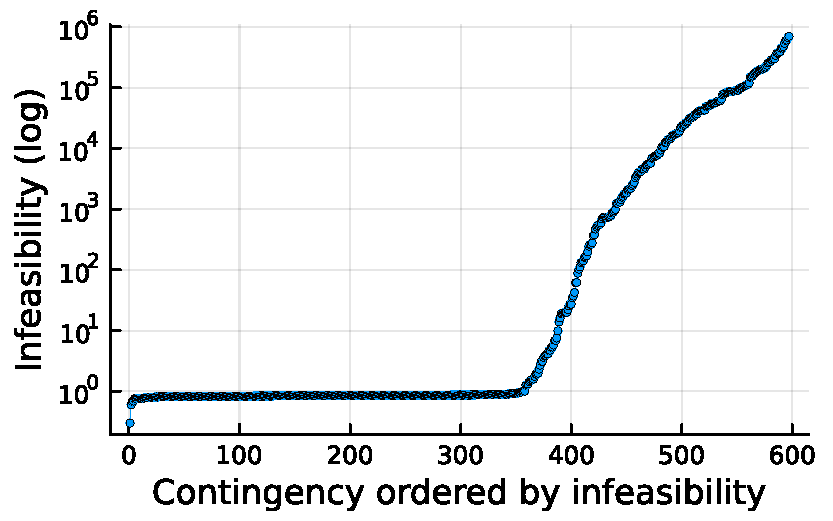
\includegraphics[width=.4\textwidth]{./figures/contingency.pdf}
\caption{Result of contingency screening for {\tt ACTIVSg500}.
The base case solution in \eqref{eq:screening} is obtained by solving
the classical OPF problem.}
\label{fig:contingency}
\end{figure}

\subsection{Solution of large-scale SCOPF}


% \subsection{Tables}
% An example of a floating table. Note that, for PSCC style tables, the
% \caption command should come BEFORE the table and, given that table
% captions serve much like titles, are usually capitalized except for words
% such as a, an, and, as, at, but, by, for, in, nor, of, on, or, the, to
% and up, which are usually not capitalized unless they are the first or
% last word of the caption. Table text will default to \footnotesize as
% IEEE normally uses this smaller font for tables.
% The \label must come after \caption as always.
%
\begin{table*}[!ht]
\centering
\caption{This is a table.}

\begin{tabular}{|rrr|rrr|rrr|rrr|}
\hline
\multicolumn{ 3}{|c|}{}  & \multicolumn{ 3}{c|}{\bf Knitro} & \multicolumn{ 3}{c|}{\bf MadNCL-CPU} & \multicolumn{ 3}{c|}{\bf MadNCL-GPU}  \\
\hline
K & nvar & ncon & Iter & Obj. & Time (s)& Iter & Obj. & Time (s)& Iter & Obj. & Time (s) \\
\hline
4 & 18400 & 24251 & 355 & 7.28 & 51.01 & 238 & 7.28 & 7.31 & 240 & 7.28 & 4.45\\
8 & 33300 & 43919 & 418 & 7.28 & 88.94 & 435 & 7.28 & 29.23 & 290 & 7.28 & 7.77\\
16 & 63100 & 83255 & 114 & 7.28 & 42.76 & 214 & 7.28 & 25.71 & 261 & 7.28 & 6.65\\
32 & 122700 & 161927 & 345 & 7.28 & 283.68 & 587 & 7.28 & 166.20 & 568 & 7.28 & 23.64\\
64 & 241900 & 319271 & 960 & 7.28 & 2159.59 & 528 & 7.28 & 273.08 & 453 & 7.28 & 27.96\\
128 & 480300 & 633959 & - & 7.29 & 4852.33 & 415 & 7.29 & 421.09 & 265 & 7.29 & 46.40\\
256 & 957100 & 1263335 & - & 7.30 & 11136.08 & 493 & 7.30 & 1120.16 & 609 & 7.30 & 170.75\\
\hline
\end{tabular}

\end{table*}


% An example is shown in Table~\ref{table_example}.
\begin{table*}[!ht]
% % increase table row spacing, adjust to taste
% \renewcommand{\arraystretch}{1.3}
\centering
\caption{This is a table.}
\begin{tabular}{|rr|rr|rrr|rrr|}
\hline
\multicolumn{ 4}{|c|}{} & \multicolumn{ 3}{c|}{\bf Knitro} & \multicolumn{3}{c|}{\bf MadNCL-GPU} \\
\hline
Name        & K   & nvar   & ncon   &  Iter & Obj. & Time (s) &  Iter & Obj. & Time (s) \\
\hline
ACTIVSg200  & 10  & 17546  & 22841  &  141  & 2.76      & 14.84    &  34   & 2.76      & 3.48     \\
ACTIVSg200  & 50  & 81906  & 106721 &  147  & 2.76      & 106.99   &  52   & 2.76      & 2.63     \\
ACTIVSg200  & 100 & 162356 & 211571 &  81   & 2.76      & 97.93    &  49   & 2.76      & 3.00     \\
\hline
ACTIVSg500  & 10  & 40750  & 53753  &  290  & 7.47      & 82.27    &  70   & 7.37      & 2.78     \\
ACTIVSg500  & 50  & 189750 & 250433 &  533  & 7.83      & 871.45   &  257  & 7.76      & 39.65    \\
ACTIVSg500  & 100 & 376000 & 496283 &  294  & 7.83      & 935.19   &  131  & 7.76      & 17.80    \\
\hline
1354pegase  & 8   & 109056 & 144327 &  43   & 7.41      & 53.82    &  36   & 7.43      & 5.08     \\
1354pegase  & 16  & 206920 & 273999 &  30   & 7.41      & 86.90    &  39   & 7.43      & 4.81     \\
1354pegase  & 32  & 402648 & 533343 &  116  & 7.41      & 656.68   &  57   & 7.41      & 12.64    \\
\hline
ACTIVSg2000 & 8   & 173024 & 229853 &  160  & 122.89    & 1442.62  &  -    & -         & -        \\
ACTIVSg2000 & 16  & 328360 & 436469 &  141  & 122.89    & 3001.10  &  747  & 122.89    & 143.28   \\
\hline
2869pegase  & 8   & 242102 & 323479 &  65   & 13.40     & 308.77   &  45   & 13.44     & 5.94     \\
2869pegase  & 16  & 459118 & 613727 &  68   & 13.40     & 775.95   &  348  & 13.40     & 75.71    \\
\hline
\end{tabular}

% \label{table_example}
% \begin{tabular}{|c|c|}
% \hline
% One & Two\\
% \hline
% Three & Four\\
% \hline
% \end{tabular}
\end{table*}

% \subsection{Figures}
% An example of a floating figure using the graphicx package.
% Note that \label must occur AFTER (or within) \caption.
% For figures, \caption should occur after the \includegraphics.
% Note that IEEEtran v1.7 and later has special internal code that
% is designed to preserve the operation of \label within \caption
% even when the captionsoff option is in effect. However, because
% of issues like this, it may be the safest practice to put all your
% \label just after \caption rather than within \caption{}.
%
%
\begin{figure}[!ht]
\centering
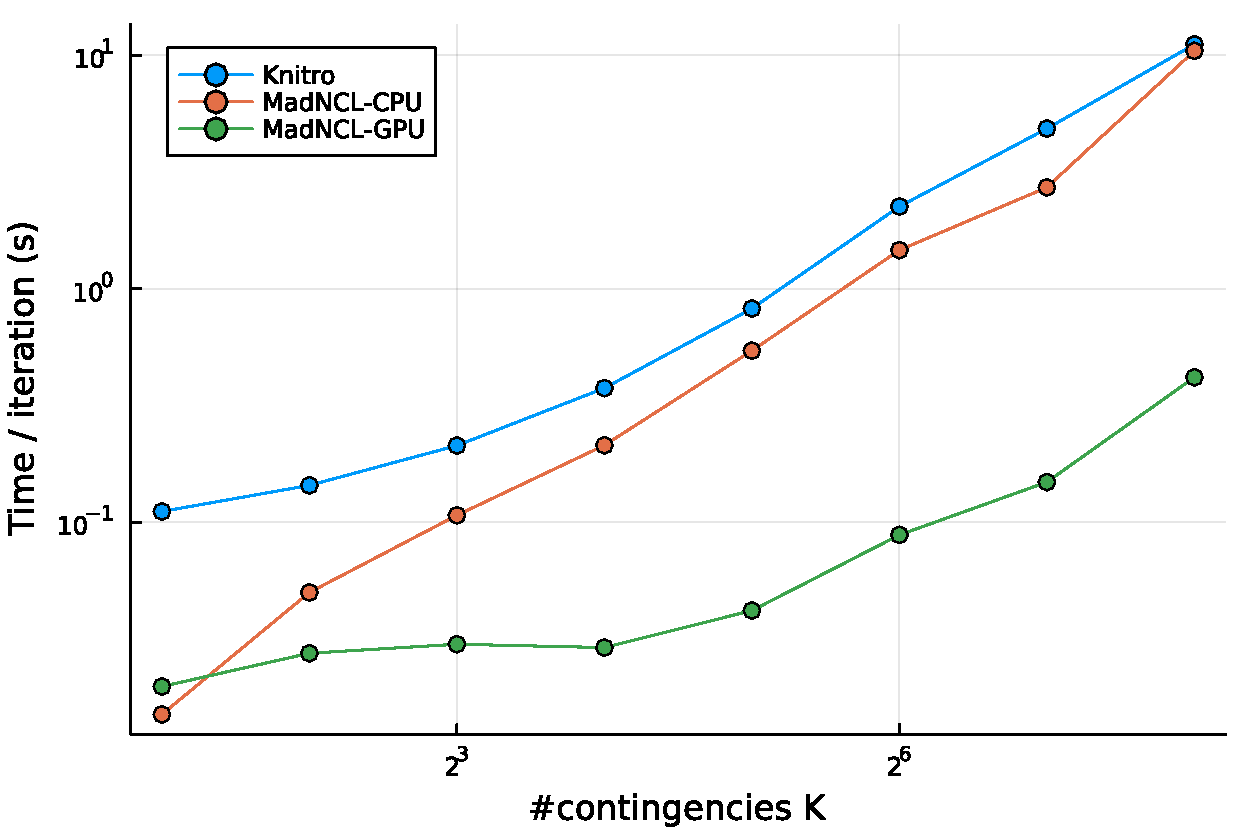
\includegraphics[width=.4\textwidth]{./figures/scalability.pdf}
\caption{Simulation results for the network.}
\label{fig:scalability}
\end{figure}

% Note that IEEE typically puts floats only at the top, even when this
% results in a large percentage of a column being occupied by floats.


% An example of a double column floating figure using two subfigures.
% (The subfig.sty package must be loaded for this to work.)
% The subfigure \label commands are set within each subfloat command,
% and the \label for the overall figure must come after \caption.
% \hfil is used as a separator to get equal spacing.
% Watch out that the combined width of all the subfigures on a
% line do not exceed the text width or a line break will occur.
%
%\begin{figure*}[!t]
%\centering
%\subfloat[Case I]{\includegraphics[width=2.5in]{box}%
%\label{fig_first_case}}
%\hfil
%\subfloat[Case II]{\includegraphics[width=2.5in]{box}%
%\label{fig_second_case}}
%\caption{Simulation results for the network.}
%\label{fig_sim}
%\end{figure*}
%
% Note that often IEEE papers with subfigures do not employ subfigure
% captions (using the optional argument to \subfloat[]), but instead will
% reference/describe all of them (a), (b), etc., within the main caption.
% Be aware that for subfig.sty to generate the (a), (b), etc., subfigure
% labels, the optional argument to \subfloat must be present. If a
% subcaption is not desired, just leave its contents blank,
% e.g., \subfloat[].





% trigger a \newpage just before the given reference
% number - used to balance the columns on the last page
% adjust value as needed - may need to be readjusted if
% the document is modified later
%\IEEEtriggeratref{8}
% The 'triggered' command can be changed if desired:
%\IEEEtriggercmd{\enlargethispage{-5in}}

% references section

% can use a bibliography generated by BibTeX as a .bbl file
% BibTeX documentation can be easily obtained at:
% http://www.ctan.org/tex-archive/biblio/bibtex/contrib/doc/
% The IEEEtran BibTeX style support page is at:
% http://www.michaelshell.org/tex/ieeetran/bibtex/
% argument is your BibTeX string definitions and bibliography database(s)
%\bibliography{IEEEabrv,../bib/paper}
%
% <OR> manually copy in the resultant .bbl file
% set second argument of \begin to the number of references
% (used to reserve space for the reference number labels box)
% \begin{thebibliography}{1}
% \bibitem{Shell}
% M.~Shell, \emph{How to Use the IEEEtran Latex Class}, Latex Archive Contents, \verb+http://www.ieee.org/conferences_events/+ \verb+conferences/publishing/templates.htm+

% \bibitem{IEEEhowto:kopka}
% H.~Kopka and P.~W. Daly, \emph{A Guide to \LaTeX}, 3rd~ed.\hskip 1em plus
%   0.5em minus 0.4em\relax Harlow, England: Addison-Wesley, 1999.




% \end{thebibliography}

\bibliographystyle{IEEEtran}
\bibliography{IEEEabrv,biblio.bib}


% that's all folks
\end{document}


